\section{Objects \& References}

\begin{frame}[plain]
What do our variables store exactly?
\end{frame}

\begin{frame}[fragile]{References}
\begin{minted}{python}
person1 = Person("Daan", "Wichmann", "Secret")
\end{minted} 

\pause
\begin{minted}{python}[breaklines]
person2 = person1
\end{minted}

\pause
\begin{minted}{python}
person3 = Person("Damai", "Jiworo", "Secret")
\end{minted} 
\end{frame}

\setbeamertemplate{caption}[numbered]
\begin{frame}{Memory model}
    \begin{figure}
        \centering
        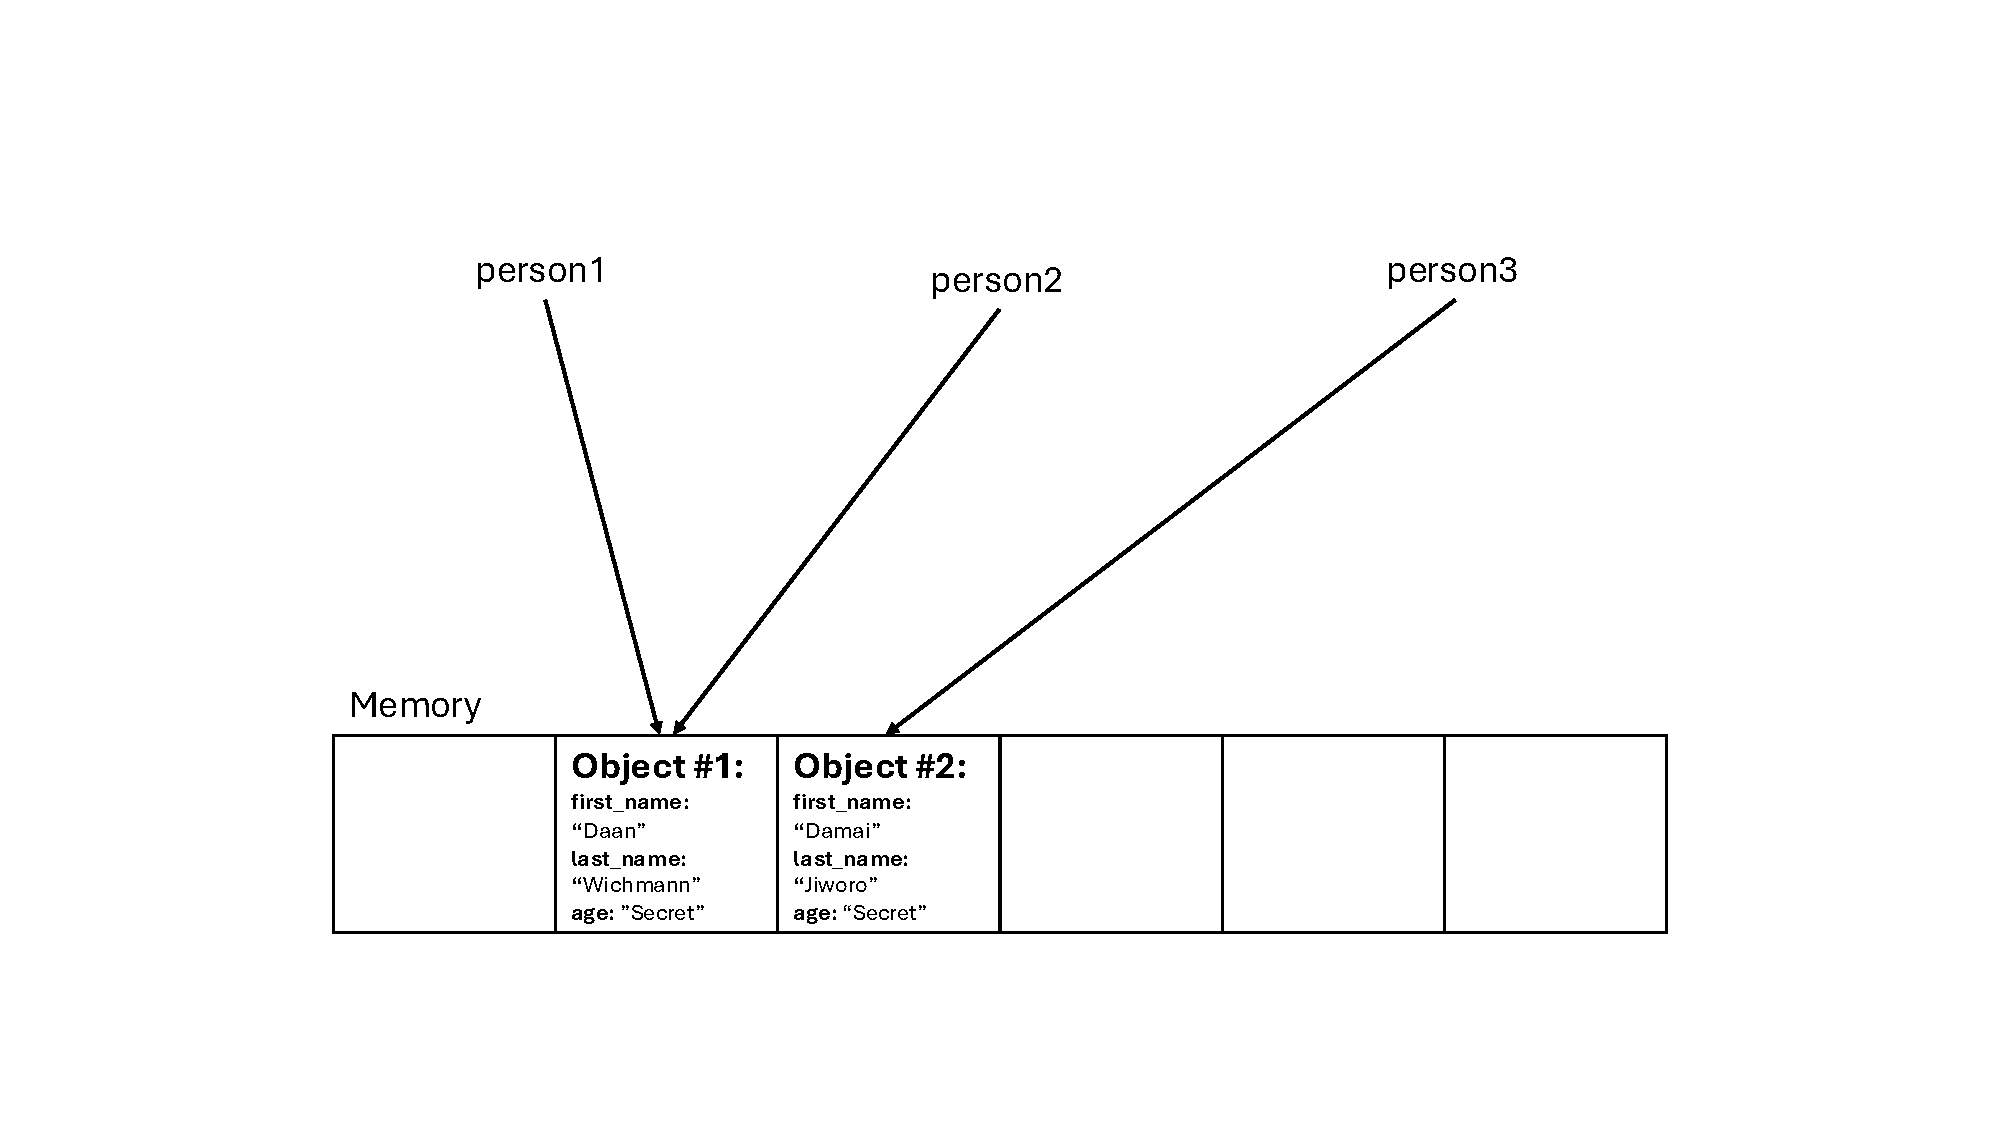
\includegraphics[scale=0.30]{images/memory.pdf}
        \caption{Simplified memory model}
        \label{fig:focuslogo}
    \end{figure}
\end{frame}

\begin{frame}[fragile]{Small quiz}
\begin{minted}{python}
person1 = Person("Damai", "Jiworo", "Secret")
\end{minted}
\pause
\begin{minted}{python}
person2 = person1
\end{minted}
\pause
\begin{minted}{python}
person3 = Person("Daan", "Wichmann", "Secret")
\end{minted} 
\pause
\begin{minted}{python}
person2.first_name = "Emma"
\end{minted}
\pause
\begin{minted}{python}
print(person1.first_name)  # What is the output?
\end{minted}
\pause
\begin{minted}{python}
>>> "Emma"
\end{minted}
\end{frame}

\begin{frame}[fragile]{Another one}
\begin{minted}{python}
person1 = Person("Damai", "Jiworo", "Secret")
\end{minted}
\pause
\begin{minted}{python}
person2 = Person("Damai", "Jiworo", "Secret")
\end{minted} 
\pause
\begin{minted}{python}
person2.first_name = "Emma"
\end{minted}
\pause
\begin{minted}{python}
print(person1.first_name)  # What is the output?
\end{minted}
\pause
\begin{minted}{python}
>>> "Damai"
\end{minted}
\end{frame}